\section{Architecture Taxonomy and Implementation}
\label{sec:architecture-taxonomy}

\subsection{Attention and Sequence-Mixer Families}
\label{sec:attention-families}

The system implements forty-four sequence mixers organized into eight functional categories that reflect how each method balances expressivity, computational cost, and memory.
\begin{enumerate}[leftmargin=*]
    \item \textbf{Dense baselines} (3): standard softmax attention, sigmoid attention, and Grouped-Query Attention (GQA) provide full global routing at quadratic cost.
    \item \textbf{Recurrent and retentive} (5): RetNet, Mamba, ODE-style blocks, and Titans maintain state for constant-time inference through recurrence, selective state spaces, continuous depth, or test-time memory.
    \item \textbf{Sparse patterns} (10): Sparse Transformer, Longformer, SWA with attention sinks, BigBird, SparseK, NSA, SpargeAttn, FASA, MSA, and SparDA reduce quadratic cost through structured sparsity, token selection, or training-free pruning.
    \item \textbf{Gated mechanisms} (8): GLA, DeltaNet, Gated DeltaNet, Gated DeltaNet-2, HGRN2, FoX, Gated Softmax, and KDA introduce data-dependent control over retention, forgetting, and update strength.
    \item \textbf{Latent compression} (10): MLA, GQLA, MLRA, Tucker, IHA, GTA, MTLA, CCA, CCGQA, and GMA compress key--value state into low-rank bottlenecks or route through a Gaussian-mixture latent memory.
    \item \textbf{Conditional memory} (1): Engram provides test-time read/write memory through learned lookups.
    \item \textbf{Fast-weight attention} (6): Falcon-1/2/3 and Falcon-1A/2A/3A treat the recurrent state transition as an online continual-learning rule \citep{zhang_falcon_2026}.
    \item \textbf{Geometric field} (1): SSOG applies a structured geometric prior over the attention matrix \citep{pisoni_ssog_2026}.
\end{enumerate}

\begin{figure}[t]
\centering
\fitfigure{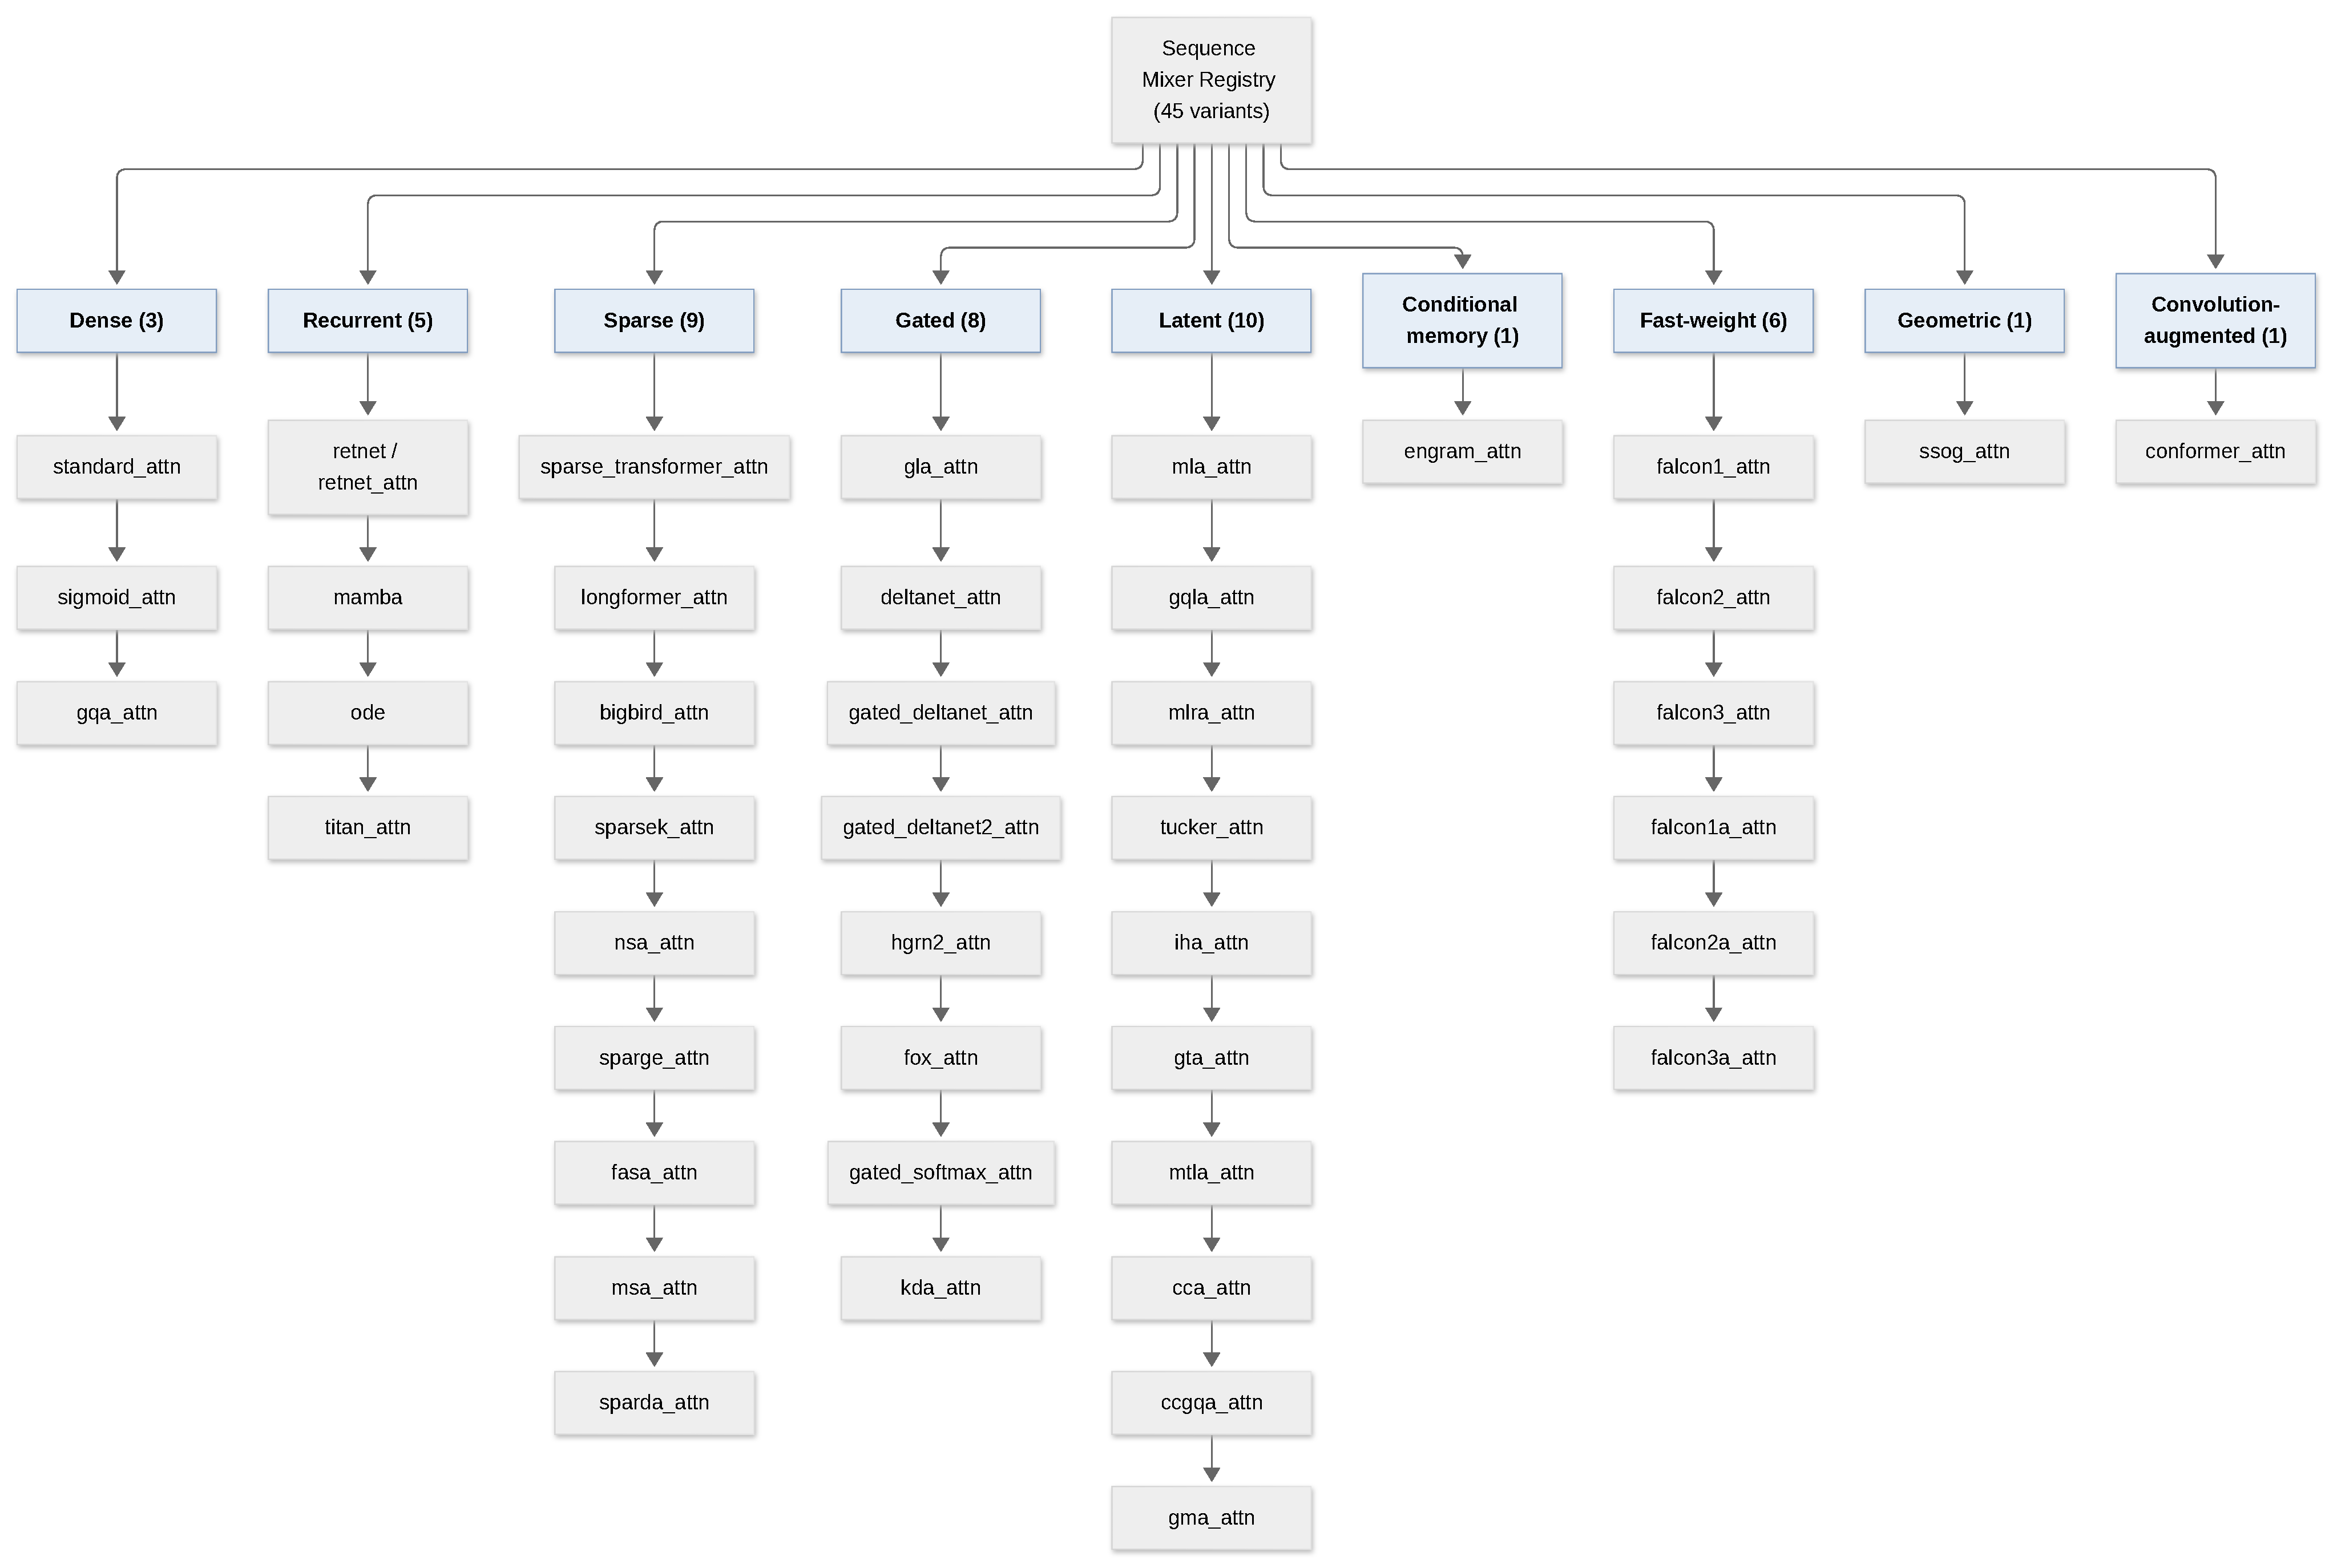
\includegraphics{figures/mixer-taxonomy.pdf}}
\caption{Taxonomy of the forty-three sequence mixers across eight functional categories. Dense baselines provide full global routing at quadratic cost; recurrent methods compress state for constant-time inference; sparse variants restrict the attention pattern; gated mechanisms modulate retention and forgetting; latent methods compress key--value representations; conditional memory adds test-time read/write lookups; fast-weight methods cast the state transition as an online learning rule; geometric methods encode structured priors.}
\label{fig:comprehensive-taxonomy}
\end{figure}

\subsection{Dense and Recurrent Families}
The dense baselines---standard softmax \citep{vaswani_attention_2017} and sigmoid attention \citep{ramapuram_theory_2024}---and the recurrent family---RetNet \citep{sun_retentive_2023}, Mamba \citep{gu_mamba_2023}, ODE-style blocks \citep{zhang_continuous_2021}, and Titans \citep{behrouz_titans_2025}---define the expressiveness-versus-efficiency trade-off. Formulations, parallel and recurrent forms, pseudocode, and a comparison table are collected in Appendix~\ref{sec:annex-transformer}.

\begin{figure}[t]
\centering
\fitfigure{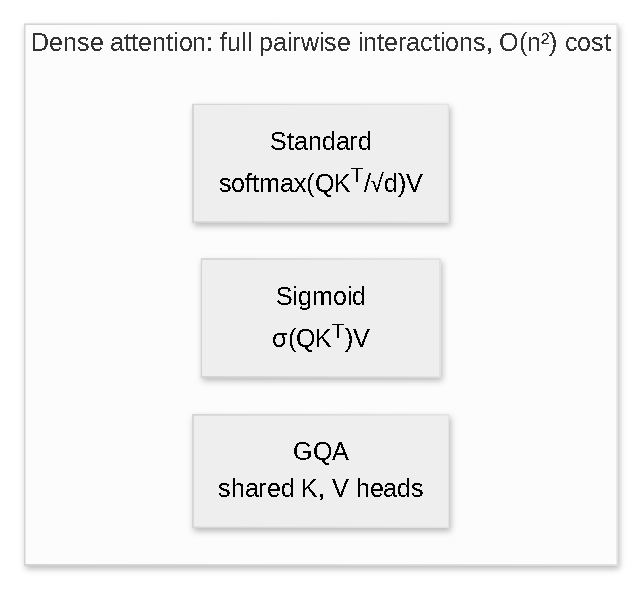
\includegraphics{figures/dense-map.pdf}}
\caption{Dense attention baselines. Standard and sigmoid attention compute full pairwise interactions; Grouped-Query Attention shares key--value heads across query groups, reducing memory traffic while keeping full attention expressivity.}
\label{fig:dense-map}
\end{figure}

\begin{figure}[t]
\centering
\fitfigure{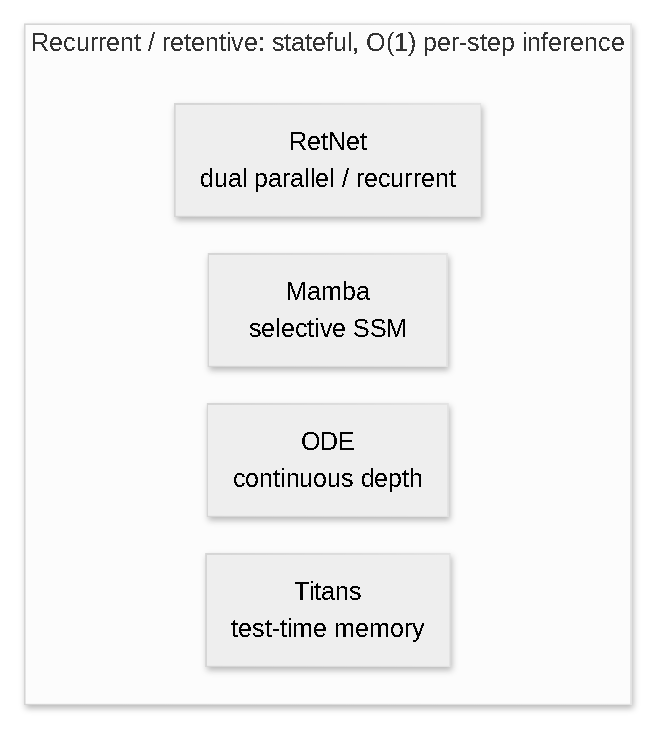
\includegraphics{figures/recurrent-map.pdf}}
\caption{Recurrent and retentive family. RetNet offers parallel and recurrent forms, Mamba uses selective state-space parameters, ODE blocks model continuous depth, and Titans add test-time memory; all achieve constant-time per-step inference.}
\label{fig:recurrent-map}
\end{figure}

\subsection{Latent and Low-Rank Attention Family}
This family compresses per-token key--value state into a low-rank latent: MLA, GQLA, MLRA, Tucker, IHA, GTA, and MTLA unify grouped-query, latent, factorized, and temporal designs. CCA and CCGQA formulate attention in a compressed latent with decoupled grouping, while GMA replaces pairwise interaction with probabilistic routing through learned Gaussian-mixture components. Formulations, pseudocode, and a comparison table are collected in Appendix~\ref{sec:annex-latent}.

\begin{figure}[t]
\centering
\fitfigure{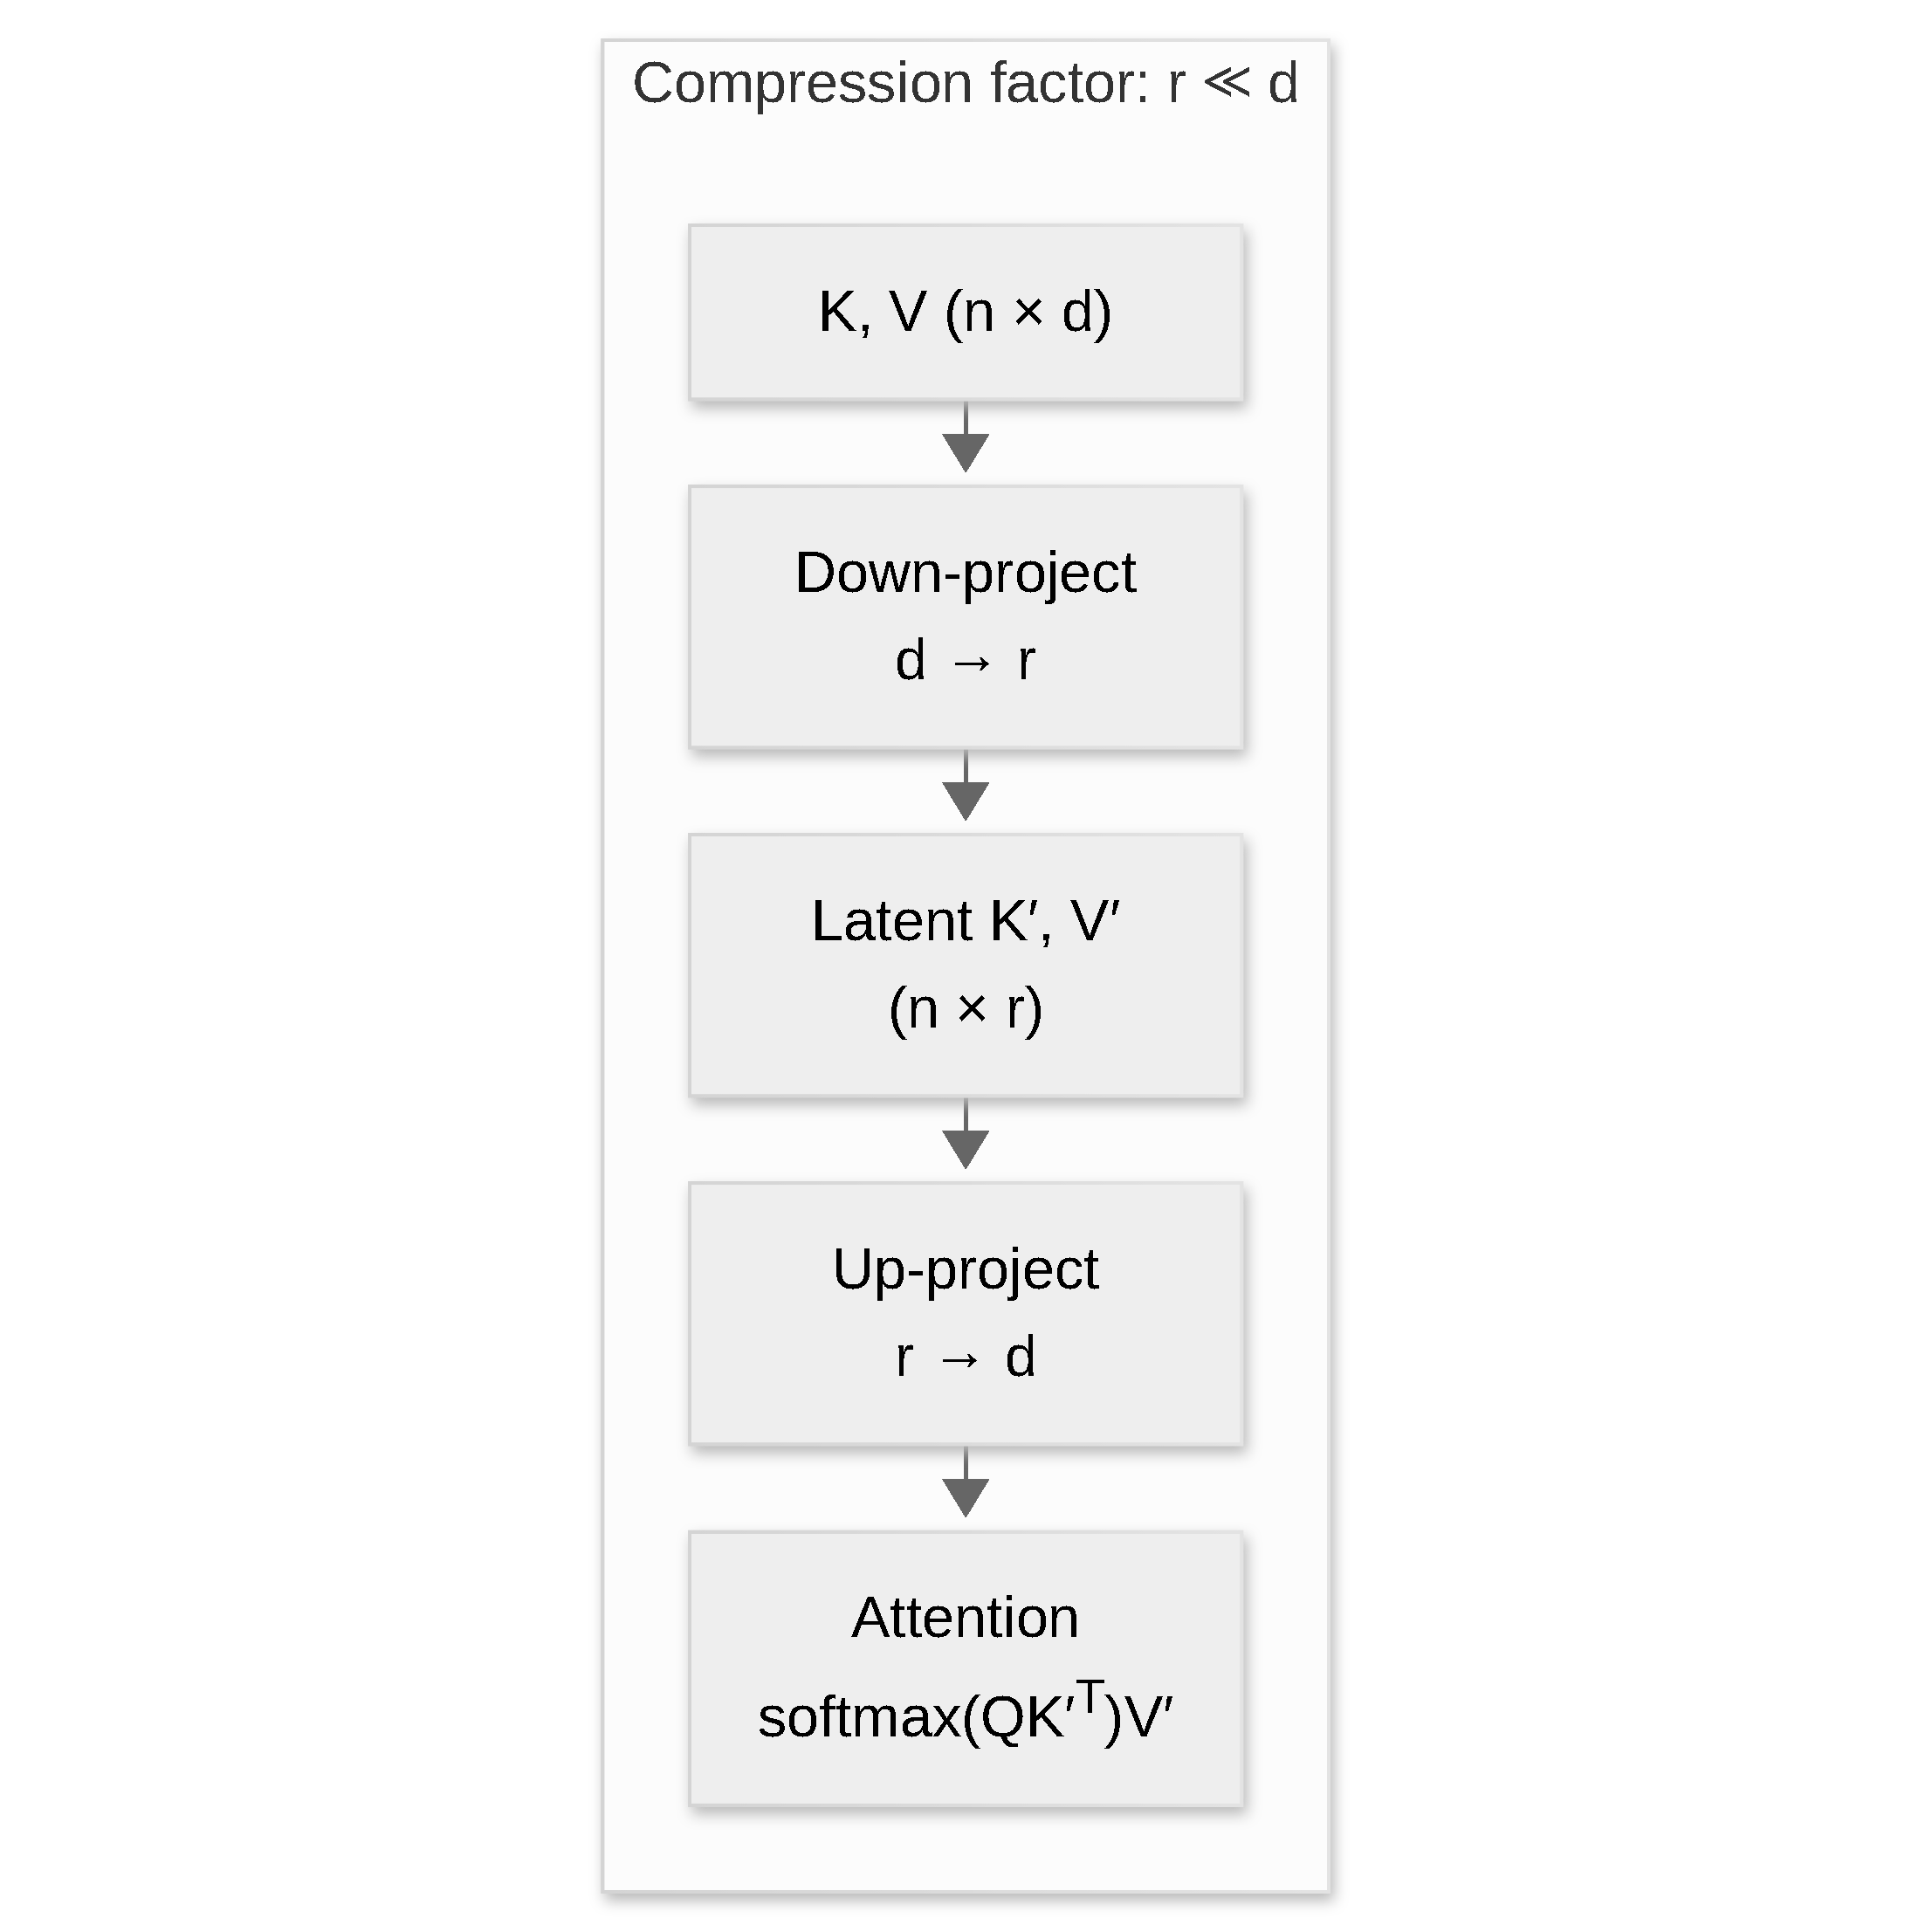
\includegraphics{figures/latent-map.pdf}}
\caption{Latent and low-rank attention. Key--value pairs are projected into a low-rank latent space, where attention is computed at reduced cost, and projected back. Variants differ in factorization, head interleaving, temporal compression, cross-covariance formulation, and probabilistic routing.}
\label{fig:latent-map}
\end{figure}

\subsection{Sparse Attention Extensions}
The registry includes ten sparse blocks \citep{child_sparse_transformer_2019,beltagy_longformer_2020,jolicoeur_sliding_window_2026,zaheer_bigbird_2020,lou_sparsek_2024,yuan_nsa_2025,zhang_spargeattn_2025,wang_fasa_2026,lai_minimax_2026,fu_sparda_2026}. Two inference-time methods, \texttt{fasa\_attn} and \texttt{sparge\_attn}, apply their sparse heuristic only when the model is in evaluation mode: during training the enclosing hybrid layer substitutes standard dense attention over the same $\mathbf{q}/\mathbf{k}/\mathbf{v}/\mathbf{o}$ projections, so the trained weights are exactly the ones the sparse path reads at inference. \texttt{swa\_attn} is also training-free but is a normal trainable mixer, so it runs its windowed pattern in both training and inference. Formulations, pseudocode, per-block characteristics, and a comparison table are collected in Appendix~\ref{sec:annex-sparse}.

\begin{figure}[t]
\centering
\fitfigure{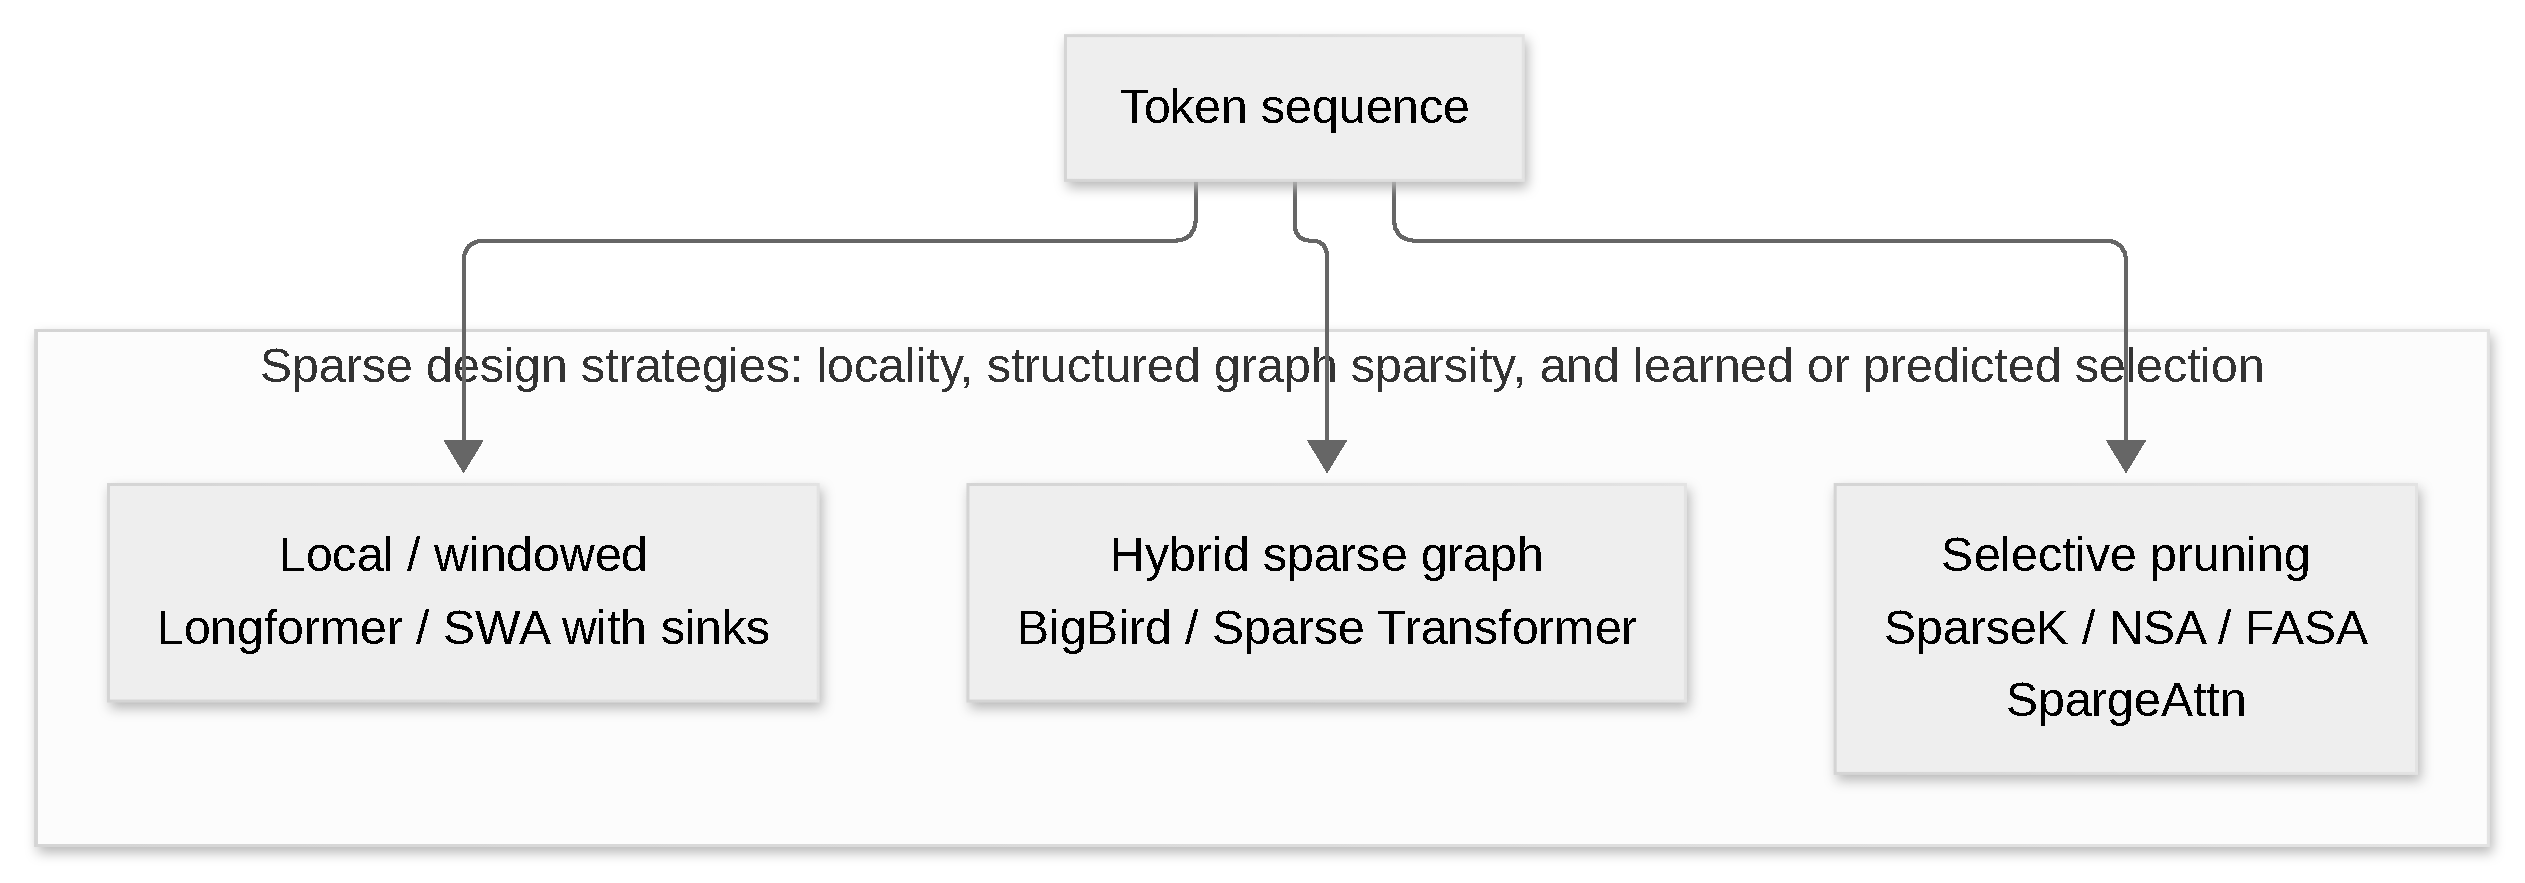
\includegraphics{figures/sparse-map.pdf}}
\caption{Sparse attention design choices. Methods reduce cost by restricting neighborhoods, constructing sparse graphs, or selecting only high-value tokens or blocks.}
\label{fig:sparse-map}
\end{figure}

\subsection{Gated and Fast-Weight Attention}
The gated family contains eight blocks \citep{yang_gla_2023,yang_deltanet_2024,yang_gated_deltanet_2024,hatamizadeh_gated_deltanet2_2026,qin_hgrn2_2024,lin_forgetting_transformer_2025,qiu_gated_attention_2025,kimi_kda_2025}. Gating controls what information survives, either in recurrent state updates (GLA, DeltaNet variants, HGRN2, KDA) or in the full attention path (FoX, Gated Softmax). Formulations, pseudocode, and a comparison table are collected in Appendix~\ref{sec:annex-gated}.

Fast-weight attention recasts the recurrent update as an online continual-learning rule; the six Falcon variants \citep{zhang_falcon_2026} unify DeltaNet-style regression and linear-attention writes under read-after-write semantics with normalized step sizes and explicit forgetting. Each variant ships a recurrent reference scan and a chunk-parallel kernel. Formulations, configuration knobs, and published results are collected in Appendix~\ref{sec:annex-fast-weight}.

\begin{figure}[t]
\centering
\fitfigure{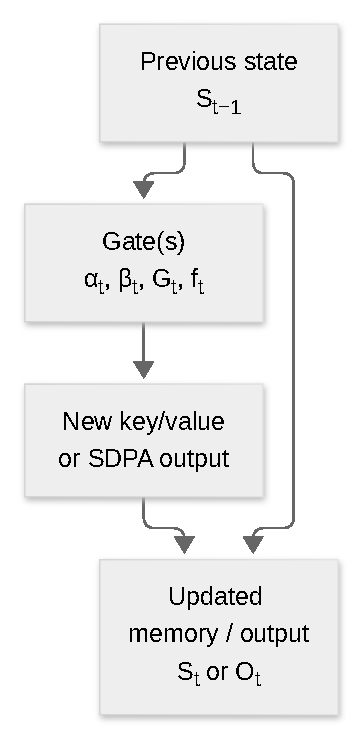
\includegraphics{figures/gating-template.pdf}}
\caption{Generic gating template. A gate can decay existing memory, regulate write strength, or modulate dense attention outputs, depending on the block family.}
\label{fig:gating-template}
\end{figure}
